% This is "sig-alternate.tex" V2.1 April 2013

\documentclass{sig-alternate-05-2015}

%----------------------------------------------------------------------------------------
%	PACKAGES AND DOCUMENT CONFIGURATIONS
%----------------------------------------------------------------------------------------
%
% please be aware to install sudo apt-get install texlive-science
%
%
\usepackage{makeidx}                    % allows for indexgeneration
\usepackage{xargs}                      % Use more than one optional parameter in a new commands
\usepackage[pdftex,dvipsnames]{xcolor}  % Coloured text etc.
% \usepackage{hyperref}
\usepackage{graphicx} 
\usepackage{enumitem}
\usepackage{scrextend}
\usepackage{pdfpages}

\usepackage{enumitem}

\usepackage{subcaption}

\usepackage[utf8]{inputenc}
\usepackage[T1]{fontenc}

\usepackage{scrextend} %for refnote
\usepackage{tabu}

\usepackage{eurosym}

\usepackage{url}
\usepackage{breakurl}
\usepackage[breaklinks]{hyperref}
\def\UrlBreaks{\do\/\do-}

% 
\usepackage[colorinlistoftodos,prependcaption,textsize=tiny]{todonotes}
\newcommandx{\unsure}[2][1=]{\todo[linecolor=red,backgroundcolor=red!25,bordercolor=red,#1]{#2}}
\newcommandx{\change}[2][1=]{\todo[linecolor=blue,backgroundcolor=blue!25,bordercolor=blue,#1]{#2}}
\newcommandx{\info}[2][1=]{\todo[linecolor=OliveGreen,backgroundcolor=OliveGreen!25,bordercolor=OliveGreen,#1]{#2}}
\newcommandx{\improvement}[2][1=]{\todo[linecolor=Plum,backgroundcolor=Plum!25,bordercolor=Plum,#1]{#2}}
\newcommandx{\thiswillnotshow}[2][1=]{\todo[disable,#1]{#2}}
%
\setlength{\parindent}{0pt}

\usepackage[numbers]{natbib}

% custom todo
%\newcommand{\todo}[1]{}
%\renewcommand{\todo}[1]{{\color{red} TODO: {#1}}}

\begin{document}

% Copyright
%\setcopyright{acmcopyright}
%\setcopyright{acmlicensed}
%\setcopyright{rightsretained}
%\setcopyright{usgov}
%\setcopyright{usgovmixed}
%\setcopyright{cagov}
%\setcopyright{cagovmixed}



%----------------------------------------------------------------------------------------
%	Meta Data
%----------------------------------------------------------------------------------------
%


\title{Simulating Strategic Interaction on Online Marketplaces}
\subtitle{[How to Survive Dynamic Pricing Competition]}



\numberofauthors{9} %  in this sample file, there are a *total*
% of EIGHT authors. SIX appear on the 'first-page' (for formatting
% reasons) and the remaining two appear in the \additionalauthors section.
%
\author{Marvin Bornstein, Johanna Latt, Jan Lindemann, Nikolai J. Podlesny, Sebastian Serth, Jan Selke}
\additionalauthors{Martin Boissier, Rainer Schlosser, Matthias Uflacker}
    

\maketitle

%
%----------------------------------------------------------------------------------------
%	Content
%----------------------------------------------------------------------------------------
%
%%%%%%%%%%%%%%%%%%%%%%%%%%     Abstract     %%%%%%%%%%%%%%%%%%%%%%%%%% 
%
%

\begin{abstract}
@TODO:\\
\end{abstract}


%\keywords{Dynamic Pricing}

%
\section{Introduction}
\label{sec:Introduction}
% Owner: Jani
% Reviewed: 
%
While for the last couple of centuries prices were mainly defined through rule-based actions, more and more companies start basing their pricing calculations and strategies on technology and data-driven processes. Not only the actual computation of profit and cost is nowadays algorithm driven, but also its update and review strategy.
One of the most competitive and advanced fields is the algorithmic trading or high-frequency trading on stock exchanges. But also, each one of us experiences nowadays technology driven price calculation on online marketplace like amazon, which we will hereinafter referred to as dynamic pricing. 

Currently, pricing strategies and algorithms exist, but handlers of those mechanism lack of the possibility to test them appropriately before releasing them into the real world where they can create huge loses \citep{uflacker2016ertragsmanagement} \citep{schlosser2016optimal} \citep{schlosser2016stochastic} \citep{schlosser2016survive}. We picked up the challenge to create such an environment, imitating different market situations and therefore testing how pricing strategies react and interact based on influences and against each other.\\

\textbf{Contribution:} In this work, we briefly elaborate our process of building a distributed and scalable platform to imitate market situations and simulate dynamic pricing algorithms and their effects with potential real world settings.
Therefore, the following Chapter \ref{sec:Architecture} contains a short introduction into the underlying architecture of the platform.
The choreography of different services is described in Chapter \ref{sec:Choreography}. Chapter \ref{sec:Behaviors} will provide insights in the already implemented algorithms and their behaviors.
A user facing interface on top of the RESTful API used for the communication between the services is delineated in Chapter \ref{sec:ui} and an evaluation of first simulations are elaborated in Chapter \ref{sec:evaluation}. Finally Chapter \ref{sec:conclusion} concludes this work. \\

%
% TODO: Do we want to keep the design goal section as standalone? And if so, we need to include it in Contribution overview of the chapters. 
% TODO: Include related work chapter in here as well if we keep it
%


%
\section{Related Work}
\label{sec:Related_Work}
% Owner: Johanna
% Reviewed: 
%
The topic of pricing competition has been widely researched and discussed in various research areas. The Bertrand-model from 1883 \citep{bertrand1883} is a very basic model looking at the situation of two companies offering one exact same product. The end result in this case according to the Bertrand-model will always be that the product will be offered at purchase price by both companies. The only differentiating feature for the customers is the price of the product, thus they will always buy the cheaper product which leads to both companies undercutting each other until they both have no profit margin left. \\

However, the situation in markets with multiple products or products with differentiating features offers a much wider variety of possible outcomes and pricing strategies. Many have researched possible pricing strategies and possible scenarios. \citet{kopalle1996} and \citet{chintagunta1996} focus on the demand as factor for dynamic pricing models, \citet{martinez2011} investigate the influence of stochastic demand, \citet{gallego2008} look at perishable products, i.e. products with a finite sales horizon, and \citet{levin2009} consider strategic consumer choices and perishable products as well. \citet{popescu2015} explored models of repricing automation in markets where products have exactly one differentiating attribute such as the seller's reputation. 

With the increasing use of online marketplaces in the last decades, the dynamic pricing topic got more and more important due to the possibility to change virtual prices within seconds, while physical prices printed on products in stores were much harder and slower to influence. But also, the consumers' behavior changes in this context as \citet{kannan2001} researched by comparing the physical value chain with the virtual-information-based value chain. \\

This showed that the consumer behavior is just as much of an important factor in dynamic pricing contexts as the pricing behavior is. However, little effort has been made to build simulation platforms that ease the development and evaluation of good pricing algorithms while taking into account all of these factors. \citet{morris2001} developed such a platform in 2001, however, it is limited in its capabilities, especially looking at huge online marketplace situations that were not the primary target context when this simulation was developed. The simulation program runs on a single machine, offers a limited set of consumer behaviors, simulates solely finite sales horizons and the pricing updates of the sellers happen only in discrete time intervals that are predefined by the system, meaning that the possibility to react on the actions of another seller are very limited. This does not represent the current situation on online marketplaces very well.

\iffalse

\begin{itemize}
    \item Bertrand (1883) model: Exact same product, two companies -> product will be offered at purchase price by both because costumers only have one differentiating feature: the price. so they buy the cheapest, no room for profit.
    
    \item Kopalle (1996): Asymmetric Reference Price Effects and Dynamic Pricing Policies  (http://pubsonline.informs.org/doi/abs/10.1287/mksc.15.1.60)
    \item Chintagunta (1996): Pricing Strategies in a Dynamic Duopoly: A Differential Game Model (https://pdfs.semanticscholar.org/d0e4/88bb8a11427853639821c7a1cba5afe57a17.pdf)
    
    \item Gallego (2008): Dynamic Pricing of Perishable Assets (https://pdfs.semanticscholar.org/d0e4/88bb8a11427853639821c7a1cba5afe57a17.pdf)
    
     \item Martinez-de-Albeniz (2011): Dynamic Price Competition with Fixed Capacities (stochastic demand, http://pubsonline.informs.org/doi/abs/10.1287/mnsc.1110.1337?journalCode=mnsc)
    
    \item Levin (2009): Dynamic Pricing in the Presence of Strategic Consumers and Oligopolistic Competition (strategic consumers, perishable products - http://pubsonline.informs.org/doi/abs/10.1287/mnsc.1080.0936)
    
   
    \item Kannan (2001): Dynamic Pricing on the Internet: Importance and
Implications for Consumer Behavior (http://www.tandfonline.com/doi/pdf/10.1080/10864415.2001.11044211?needAccess=true)
Under Competition

    \item Morris (2001): A Simulation-based Approach to Dynamic Pricing  (developed simulation, however only locally running program, rather inflexible, given limited set of consumer behaviors, certain restrictions on the products - only finite, price updates only in ticks, not yet targeted at highly dynamic online marketplaces) https://dspace.mit.edu/bitstream/handle/1721.1/29169/49676094-MIT.pdf;sequence=2) 
\end{itemize}

%Check literature review in \url{http://faculty.chicagobooth.edu/workshops/omscience/pdf/Spring%202016/Popescu.pdf}

\fi

\section{Design Goals}
\label{sec:Design_Goals}
% Owner: Johanna
% Reviewed: 
%
Given the current, very limited possibilities to simulate a huge, dynamic online marketplace, we came up with a set of specific design goals and restrictions, that we wanted to fulfill to make the platform and the resulting simulation as realistic, dynamic and reactive as possible: 
\begin{itemize}
    \item \textbf{Reactivity:} Allow pricing algorithms to do fully dynamic price updates and look-ups at any time without being refrained by discrete time intervals to enable truly reactive pricing strategies.
    \item \textbf{Security:} Prevent fraud in simulation setups with multiple participants to allow the simulation to be used for competitions or education purposes. Fraud could be the deliberate influence on the expenses or profits of other pricing algorithms or the usage of data (e.g. for learning purposes) that is normally not accessible.
    \item \textbf{Realism:} Enforce real-life restrictions present in every big real-life marketplace such as a limited amount of price updates per time interval to avoid advantages by constantly changing prices.
    \item \textbf{Flexibility:} Offer the greatest possible flexibility in terms of scalability and adaptivity of the system to make the system easily expandable and adaptable to new possible design goals or user needs. 
\end{itemize}

\section{Architecture}
\label{sec:Architecture}
% Owner: Jani
% Reviewed:
%
Confronted with the challenge of creating a high-performance and expandable infrastructure for simulating a marketplace with different merchants and consumers, a microservice architecture was created allowing the user to scale, exchange or add single service ad-hoc and on demand. Each service within our architecture implements one business artifact. This architecture pattern comes with the cost of a communication overhead and requires farsighted API design.\\

Figure~\ref{fig:fmc} describes the underlying architecture modeling as FMC\footnote{\url{http://www.fmc-modeling.org/}} diagram. When initiating a new simulation universe, it comes along with the marketplace component, as well as the producer and a management ui for controlling each service. While the producer offers products, the marketplace holds the current market situation and handles price updates and purchases of goods. Each transaction handled by the producer and marketplace is logged to a stream database, namely Apache Kafka\footnote{\url{https://kafka.apache.org/}}. Further, those logs are being analyzed and aggregated through a batch data processing component which is in our case Apache Flink\footnote{\url{https://flink.apache.org/}} and written back into a new Kafka topic. Those details, then, can be accessed through a socket connection or REST interface provided by a kafka-reverse-proxy. 
To liven the place up, numerous consumers or merchants may join and participate in this market simulation. By default, one consumer and five\todo{are it really five?} merchants are deployed with already implemented strategy. Those behaviors are deepened in chapter \ref{sec:Behaviors} while the choreography of the single services is delineated in chapter \ref{sec:Choreography}.

%
\begin{figure}[h]
    \centering
    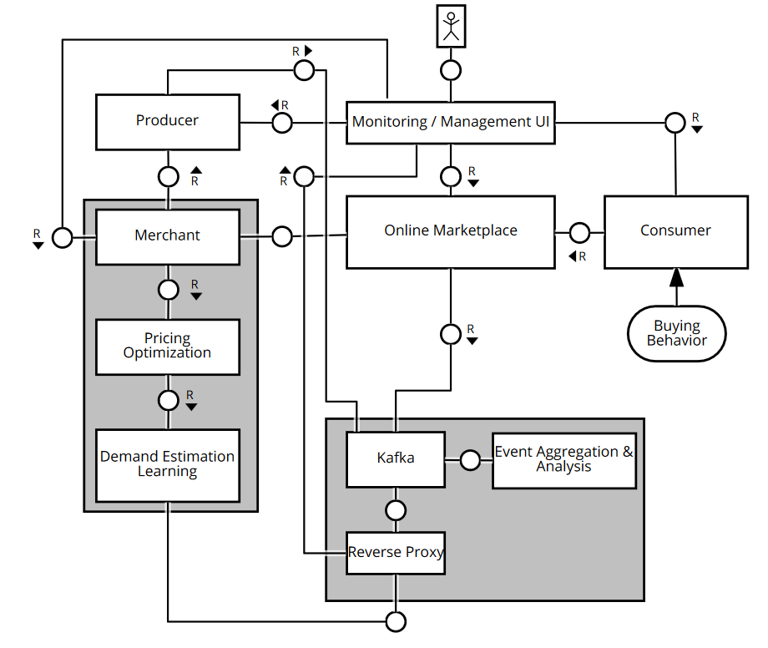
\includegraphics[width=0.5\textwidth]{images/architecture_fmc.png}
    \caption{FMC diagram of the Price Wars architecture}
    \label{fig:fmc}
\end{figure}
%
\section{Service Choreography}
\label{sec:Choreography}
% Owner: Seb
% Reviewed: jani
%
Like previously discussed, the architecture consists out of several services communicating with each other. This communication is done via well-defined RESTful APIs using JSON objects\footnote{\url{https://hpi-epic.github.io/masterproject-pricewars/}}.  Due to the micro-service architecture and the design goal to allow real competition of different merchants without cheating, all important routes are secured by authorization tokens. For authenticating all participants in the simulation without the need of a centralized authentication server, a hash-based token and identification system was introduced which additionally enables the id based logging of event message corresponding to one merchant or consumer. One of the causes to implement this decentralized authentication system was to reduce the amount of requests during the simulation. Described in the previous section, the gain of flexibility and scalability of services withing a microservice architecture goes along with the cost of an increased communication overhead. With this knowledge and experiences of a first prototype, the goal was to reduce the amount of request being sent over the network for streamlining a simulation and its necessary communication. 
In the following, we will briefly outline some of the main challenges which were solved.

\subsection{Decentralized Authorization}
\subsection{Event log analysis with Kafka and Flink}
\subsection{Challenges with high-density inter-service communication}
\subsection{Simulation Limits and bottleneck evaluation}

@TODO: how do the services interact, how do we secure some major challenges in short sentences.

No ticks or such, but completely free and dynamic, every merchant can check or update prices at any time -> close to real life (unlike eg http://www.informsrmp2017.com/description-challenge.pdf)

\begin{itemize}
\item event logs, kafka etc
\item fraud / cheating (and explain, why the consumer is required to send the price when buying products)
\item (inter service communication (via REST and connection pools))
\item (where are limits / bottlenecks?)
\end{itemize} 

@Todo: include data
Simulation 1 Stunde, 4000 Produkte à 4 Qualitäten, max 1000 Aktionen (Updates / Käufe) pro Minute, 750 Offer pro Merchant
06: 25 MB
05: 2,3 GB
04: 24 MB
03: 4 MB
02: 2 MB
01: 60 KB
\section{Behaviors}
\label{sec:Behaviors}
% Owner: Jani
% Reviewed:
%
The addressed solution provides in its default setting already several behaviors for merchants as well as the consumers. The former include known rule-based strategies like the ``Gas Station strategy'', ``Be the n-cheapest'', ``fix pricing'' as well as a first data-driven approach implementing a pricing strategy based on logistic regression \citep{hosmer2013applied}.

%
\begin{figure}[h]
    \centering
    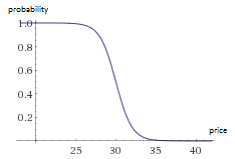
\includegraphics[width=0.25\textwidth]{images/sigmoid.png}
    \caption{Sigmoid distribution as consumer behavior}
    \label{fig:sigmoid_distribution}
\end{figure}
%

Additionally, a consumer is included in the deployment implementing several buying behaviors which can be chosen, weighted and reconfigured on-the-fly. Those behaviors range from very subtle approaches like buying the n-cheapest, first, most expensive or simple random offers on the marketplace up to more sophisticated methods trying to imitate more complex consumer situations. A sigmoid distribution with twice of the producer price as mean (see fig. \ref{fig:sigmoid_distribution}) is available through the default settings as well as a logit behavior.

The logit behavior implements a logistic regression with feature scaling and calculates for each offer the buying probability based on the feature coefficients provided in the behavior settings. Based on this buying probability for each offer, the consumer will actually choose an offer to buy. In this way, potential consumer behavior can be learned on real world data and imitated in the simulation solution.

The default settings for the logit behavior holds coefficients which were extracted from a real world use case provided by a big book retail company. For deeper insights in the concepts of logistic regression, the reader is kindly referred to \citet{hosmer2013applied} elaboration.

%
\begin{figure}[h]
    \centering
    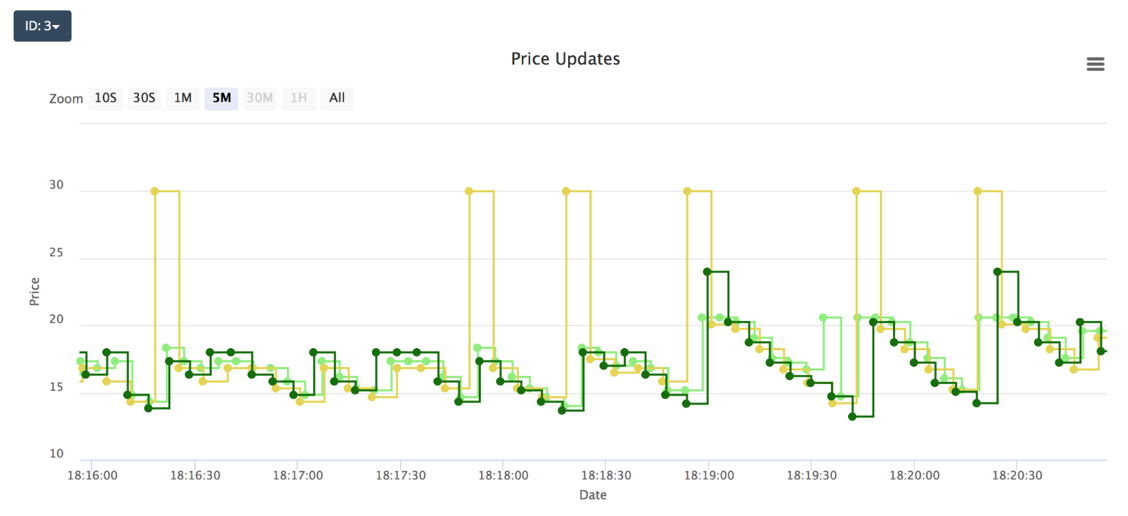
\includegraphics[width=0.5\textwidth]{images/price_graphs_v2.png}
    \caption{Price Graphs}
    \label{fig:price_graphs_v2}
\end{figure}
%

%
\subsection{Logistic Regression}
\label{sec:Logistic_Regression}
% Owner: 
% Reviewed:
%
Logistic regression is a regression model where the dependent variable -- in our case the selling of an offer -- is categorical. This categorization outcome must be discrete and should be dichotomous in nature simply expressed by a boolean whether a purchase happened or not. To determine this, this behavior consumes features and their coefficients can be altered within runtime and will then be applied to the next calculation iteration taking place. The describing hashmap of features and their coefficients contains only available features which are already implemented otherwise they will be ignored.
\section{User Interface}
\label{sec:ui}
% Owner: Jani, Johanna
% Reviewed: 
%
The ``Management User Interface'' (UI) enables the user to configure, operate and orchestrate the different microservices all in one place. 

Consuming the RESTful APIs exposed by each individual service, we use websockets to realize a a real-time streaming connection to the kafka-reverse-proxy component that provides the UI with all necessary data.

%Its implementation is based on angularJS consuming the RESTful APIs exposed by each individual service. Additionally, we used the socket.io\footnote{\url{https://github.com/socketio/socket.io}} technology which imitates a websocket connection based on HTTP to realize a real-time streaming connection to the kafka-reverse-proxy as consumer of the Apache Kafka\footnote{\url{https://kafka.apache.org/}} instances.

%Consuming the RESTful APIs exposed by each individual service, we additionally used websockets to realize a real-time streaming connection to the kafka-reverse-proxy as consumer of the Apache Kafka\footnote{\url{https://kafka.apache.org/}} instances.

The UI allows a user of the simulation to start and stop a simulation in the sense that all components having a state can be started, stopped, accessed and configured here, including their state. These components are the merchants and the consumer. Furthermore, all exposed settings for the behavior of each merchant and the consumer can be viewed, edited and updated.

The stateless components of the simulation, such as the producer and the marketplace, cannot be stopped or started, but configured here as well. E.g., products can be added or deleted, or the marketplace can be emptied with the necessary login-credentials for the underlying database.

If a user wants to register a new merchant and send it into the simulation, they can use the UI to register a new endpoint under which the merchant is running, and in return receive a secret token that is used for authorization (rf. \cref{sec:DecentralizedAuthorization}). 

Furthermore, the UI also offers easy access to visualizations of the real-time pricing interaction of merchants and to key performance indicators of each merchant, simplifying the process of comparing different pricing strategies.
\newpage 
\section{Conclusion}
\label{sec:conclusion}
% Owner:
% Reviewed:

Lorem ipsum dolor sit amet, consetetur sadipscing elitr, sed diam nonumy eirmod tempor invidunt ut labore et dolore magna aliquyam erat, sed diam voluptua. At vero eos et accusam et justo duo dolores et ea rebum. Stet clita kasd gubergren, no sea takimata sanctus est Lorem ipsum dolor sit amet. Lorem ipsum dolor sit amet, consetetur sadipscing elitr, sed diam nonumy eirmod tempor invidunt ut labore et dolore magna aliquyam erat, sed diam voluptua. At vero eos et accusam et justo duo dolores et ea rebum. Stet clita kasd gubergren, no sea takimata sanctus est Lorem ipsum dolor sit amet.

The source code and the documentation will be publicly available at\\
\url{https://github.com/hpi-epic/masterproject-pricewars} \\
while screencasts are accessible under\\
\sloppy
\url{https://www.youtube.com/watch?v=75dStkQiYNo},  
\url{https://www.youtube.com/watch?v=sdo328JU_0Y}, and
\url{https://www.youtube.com/watch?v=YJG9fGpJU_8}.\\

%\end{document}  % This is where a 'short' article might terminate

%\newpage

%ACKNOWLEDGMENTS are optional
\section*{Acknowledgments}
As part of this elaboration, special thanks goes to Dr. Matthias Uflacker, Dr. Rainer Schlosser and Martin Boissier for their continuous support and supervision. Also, we thank all attendant members of the EPIC research group for their fruitful discussions.


\bibliographystyle{unsrtnat}
\bibliography{bibtex/references.bib}  


\end{document}
